\appendix
\section{GMRES}\label{appendix:GMRES}

The Generalised Minimum Residual Method (GMRES) \cite{Saad1986GMRES:Systems} is a iterative method based on Krylov methods for solving the System $A\bm{x}=\bm{b}$ where $A$ is an arbitary non-symmetric matrix of order $n$ and $\bm{b}$ is a known vector of order $n$. Krylov methods generate a Krylov subspace through repeativly performing vector matrix multiplication involving $A$, this allows for the computation of large systems where operation of order $\mathcal{O}(n^3)$ are too large to compute the matrix inverse or where we are unable to form the matrix by can compute the matrix vector product as in the Kernel Independent Fast Multiple Method (KIFMM) (\cref{sec:KIFMM}) \cite{Ipsen1998TheMethods}.
At each iteration $k \geq 1$ find the solution $\bm{y}_k$ from the subspace 
\begin{equation*}
    \mathcal{K}_k(A,v^{(0)}) = \text{span}(\bm{v}^{(0)},A\bm{v}^{(0)},A^2\bm{v}^{(0)},\dots,A^{k-1}\bm{v}^{(0)})
\end{equation*}
where $\bm{v}^{0}$ is the normalised vector of the residual $\bm{r}^{(0)}=\bm{b}-A\bm{x}^{(0)}$ which reduces the residual to the least square problem $\min\limits_{x\in\mathcal{K}(A,b)} \lVert b-Ax \rVert$. When no initial guess $\bm{x}^{(0)}$ is given we have that $\bm{r}^{(0)}=b$, experimental results for when an initial guess is provided can be seen in \cref{sec:Guess}. GMRES solves this least square problem through the use of a orthogonal basis $\{\bm{v}^{(1)},\bm{v}^{(2)},\dots,\bm{v}^{(k)}\}$ for $\mathcal{k}(A,b)$, this is constructed using Arnoldi's method \cite{Arnoldi1951TheProblem,Elman2005FiniteDynamics}. The $k+1$ subspace is constructed from the $k$ subspace by orthogonalising the vector $A\bm{v}_K$ vector against $\mathcal{K}_k(A,v^{(0)}$ subspace. This is done by
\begin{equation*}
    \bm{\hat{v}}_{k+1} = A\bm{v}_k - (h_{1,j}\bm{v}_1 + \dots + h_{j,j}\bm{v}_j)
\end{equation*}
where $h_{ij} = v_j^*Av_j$ where is the conjugate transpose of $v_j$. We then normalise $\bm{\hat{v}}_{k+1}$ to obtain $\bm{v}_{k+1}=\bm{\hat{v}}_{k+1}/\lVert \bm{\hat{v}}_{k+1} \rVert$
By collecting the basis vectors in a matrix $V_k = [\bm{v}^{(1)},\bm{v}^{(2)},\dots,\bm{v}^{(k)}]$ we get that the decomposition from Arnoldi's method as
\begin{equation*}
    AV_j = V_{j+1} H_j
\end{equation*}
 where $H_j$ is an upper Hessenberg matrix of size $j + 1\times j$ formed by $\hat{H}_k = [h_{ij}]_{1 \leq i \leq k+1, 1 \leq j \leq k}$. As our solution to the least square problem is in $\mathcal{K}_k(A,r^{(0)})$ then we can write it as $V_k\bm{y}^{(k)}$ for some vector $\bm{y}^{(k)}$. This means we can rewrite the least problem in terms of $H_k$ as
 \begin{equation*}
 \begin{aligned}
          \beta_k &= \min\limits_{\bm{y}^{(k)}} \lVert  \beta_0 \bm{v}_0 - AV_k\bm{y}^{(k)} \rVert \\
          &= \min\limits_{\bm{y}^{(k)}} \lVert \beta_0 V_{k+1} \bm{e}_1 - V_{k+1}H_k\bm{y}^{(k)} \rVert \\
          &= \min\limits_{\bm{y}^{(k)}} \lVert \beta_0 \bm{e}_1 - H_k\bm{y}^{(k)} \rVert
 \end{aligned}
 \end{equation*}
where $\bm{e}_1 = [1,0,\dots,0]^T$. This process is repeated until $\beta_k$ is under some relative tolerance $\tau$ specified. The final estimation for $\bm{x}$ is therefore constructed from $\bm{x}^{(k)} = \bm{x}^{(k)} + V_k\bm{y}^{(k)}$.
\begin{algorithm}
\caption{The GMRES Algorithm}\label{alg:GMRES}
\begin{algorithmic}[1]
\State Choose $\bm{x}^{(0)}$, compute $\bm{r}^{(0)}=\bm{b}-A\bm{x}^{(0)}$, $\beta_0 = \lVert \bm{r}^{(0)} \rVert$, $\bm{v}^{(0)} = \bm{r}^{(0)}/\beta_0$
\For{$k = 1,2,\dots \textbf{ Until } \beta_k < \tau \beta_0$}
\State $\bm{w}_0^{(k+1)} = Av^{(k)}$
\For{$l = 1$ to $k$}
\State $h_{lk}=\langle \bm{w}_l^{(k+1)}, \bm{v}^{(l)} \rangle$
\State $\bm{w}_{l+1}^{(k+1)} = \bm{w}_l^{(k+1)} - h_{lk}\bm{v}^{(l)}$
\EndFor
\State $h_{k+1,k}=\lVert \bm{w}_{k+1}^{(k+1)} \rVert$
\State $\bm{v}^{(k+1)} = \bm{w}_{k+1}^{(k+1)}/h_{k+1,k}$
\State Compute $\bm{y}^{(k)}$ such that $\beta_k = \lVert \beta_0 \bm{e}_1 - H_k  \bm{y}^{(k)} \rVert$ is minimised, where
\State $H_k = [h_{ij}]_{1 \leq i \leq k+1, 1 \leq j \leq k}$
\EndFor
\State $\bm{x}^{(k)} = \bm{x}^{(k)} + V_k\bm{y}^{(k)}$, where $V_k = [\bm{v}^{(1)},\bm{v}^{(2)},\dots,\bm{v}^{(k)}]$
\end{algorithmic}
\end{algorithm}

GMRES will converge on the least square solution in at most $n$ iterations, although will often converge to small values of $\beta_k$ in less steps. The exact number of iteration is correlated closely with the  condition of the matrix $A$ where better conditioned matrices will converge quicker. In slow converging systems, where the number of iterations $k$ required to converge to the required tolerance $\tau$ is large can result in large computation and storage requirements as the new vector $\bm{v}_{k+1}$ needs to be orthogonalised against all previous vectors in the basis. This means that the computation and storage requirements for the GMRES algorithm grows like $\mathcal{O}(kn)$. An adaption to the algorithm denoted GMRES($m$) is used where after $m$ iterations the best guess $\bm{u}^{(m)}$ is constructed and used in place of $\bm{u}^{(0)}$ as the initial guess. This provides a upper bound on the computation and storage requirement of the algorithm although may slow down convergence as each approximation is built using a smaller Krylov subspace.

\section{Tree traversal}\label{appendix:Tree}
In this section we will give a brief overview of the two tree traversals needed to preform the fast multiple algorithm. We will concider a simple binary tree where each node had two children nodes. If we concider the binary tree in \cref{fig:BlankTree}, then we can consider both pre and post order traversal.
\begin{figure}[ht]
    \centering
    \resizebox{.4\linewidth}{!}{\begin{tikzpicture}
    \node[anchor = south west,inner sep=0] (image) at (0,0) {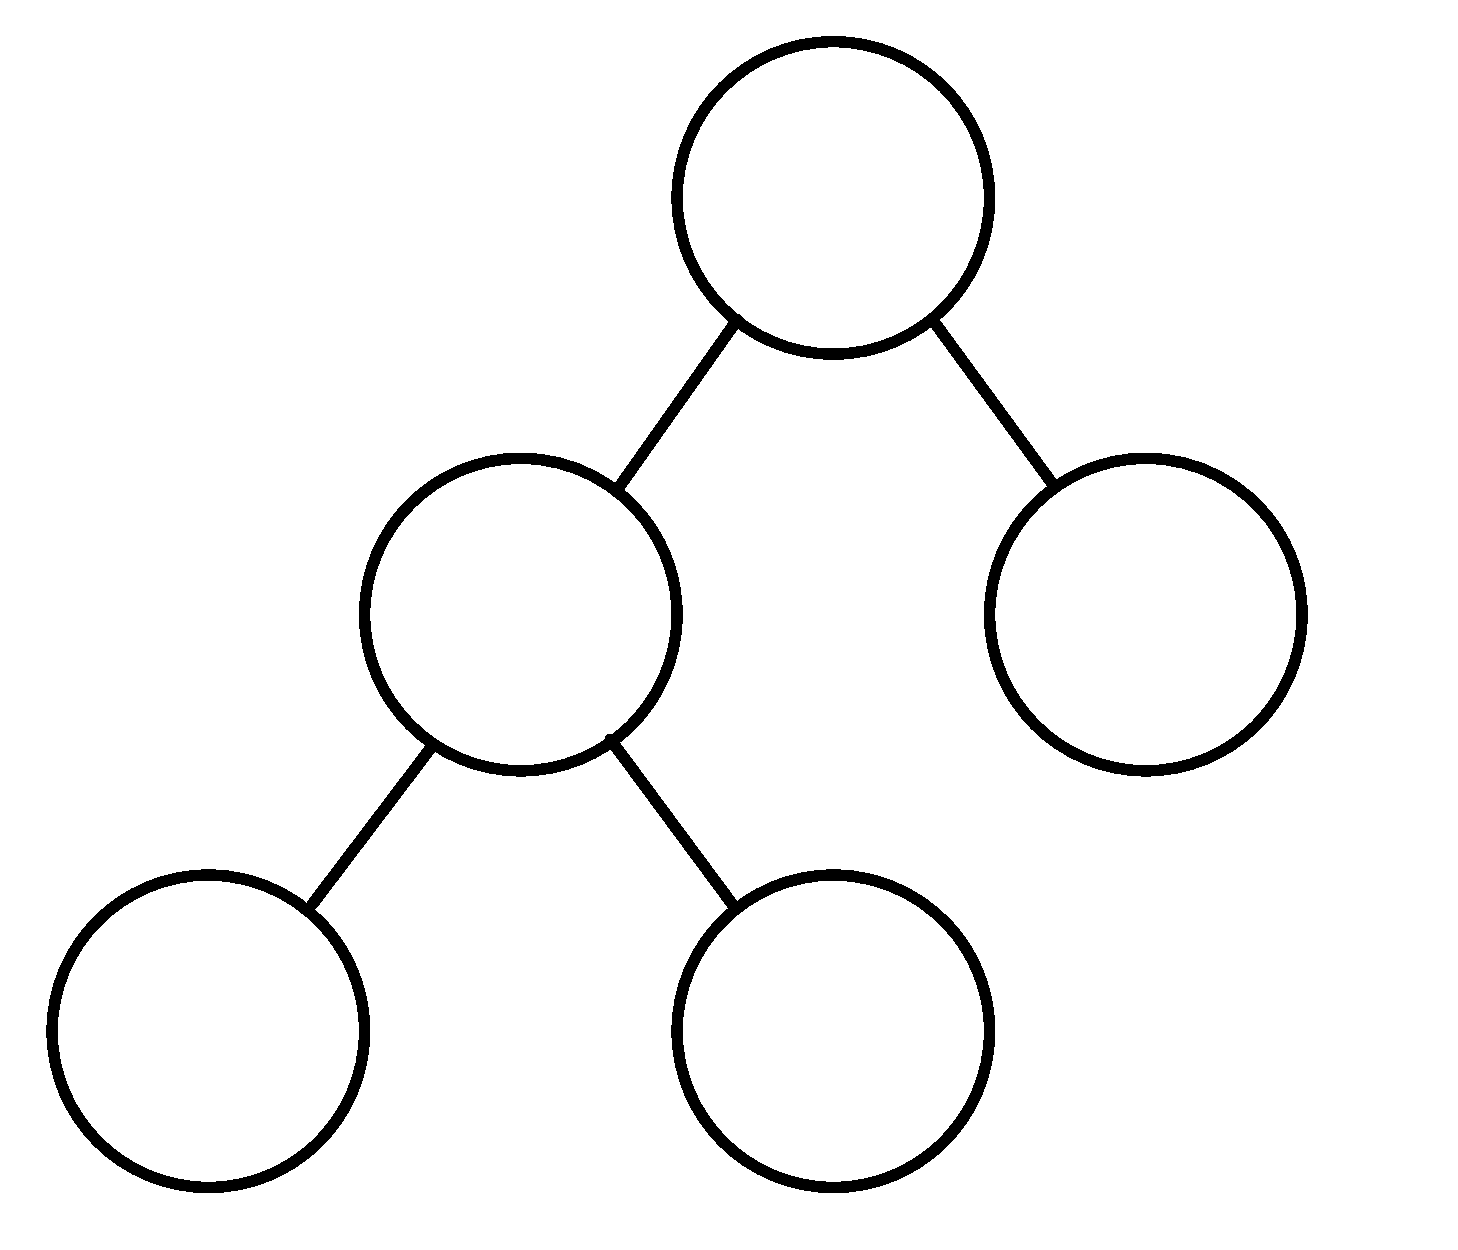
\includegraphics[width=.6\textwidth]{Images/TreeTraversal/BlankTree.pdf}};
    \begin{scope}[x={(image.south east)},y={(image.north west)}]
    \begin{scope}[x={(image.south east)},y={(image.north west)}]
        \node at (0.57,0.83) {\Huge $1$};
        \node at (0.36,0.51) {\Huge $2$};
        \node at (0.78,0.51) {\Huge $3$};
        \node at (0.14,0.17) {\Huge $4$};
        \node at (0.57,0.17) {\Huge $5$};
    \end{scope}
    \end{scope}
\end{tikzpicture}}
    \caption{A simple tree structure}
    \label{fig:BlankTree}
\end{figure}
The post order traversal is used in cases where we need to look at all the children of a node before looking at the node its self. This is useful for example in the upwards pass of fast multipole method where we need to compute the upwards equivilent surface of all node before computing the upwards equivilent surface of the node its-self with the multipole to multipole translation (\cref{eq:M2M}). For the tree defined in the case of the binary tree in \cref{fig:BlankTree} we traverse the nodes in the order $4, 5, 2, 3, 1$ with the path taken displayed in \cref{fig:Postorder}. Recursivly we can define this for a binary tree as
\begin{algorithm}
\caption{Binary post-order Traversal}
\begin{algorithmic}[1]
\State Recursively traverse the current node's left subtree
\State Recursively traverse the current node's right subtree
\State Visit the current node.
\end{algorithmic}
\end{algorithm}


Another way in which we can traverse tree structures in the pre-order traversal where we work our way down from the root of the tree. We use this in fast multipole methods so we can use local to local translation (\cref{eq:L2L}). The pre-order traversal differs from post-order traversal as we visit the current node first before recursivly traversing each subtree. For example the tree in \cref{fig:BlankTree} can be traversed using pre-order traversal in the order $1, 2, 4, 5, 3$ as illistrated in \cref{fig:Preorder}. The algorithm discribing pre-order traversal is
\begin{algorithm}
\caption{Binary pre-order Traversal}
\begin{algorithmic}[1]
\State Visit the current node
\State Recursively traverse the current node's left subtree
\State Recursively traverse the current node's right subtree.
\end{algorithmic}
\end{algorithm}

Application of both traversal to an octree traversal where we traverse each subtree individually, the order in which each subtree is traversed does not matter only only comes down to convention, however we do need to make sure that every subtree is traversed for each node.


\begin{figure}
     \centering
     \begin{subfigure}[b]{0.45\textwidth}
         \centering
         \resizebox{\linewidth}{!}{\begin{tikzpicture}
    \node[anchor = south west,inner sep=0] (image) at (0,0) {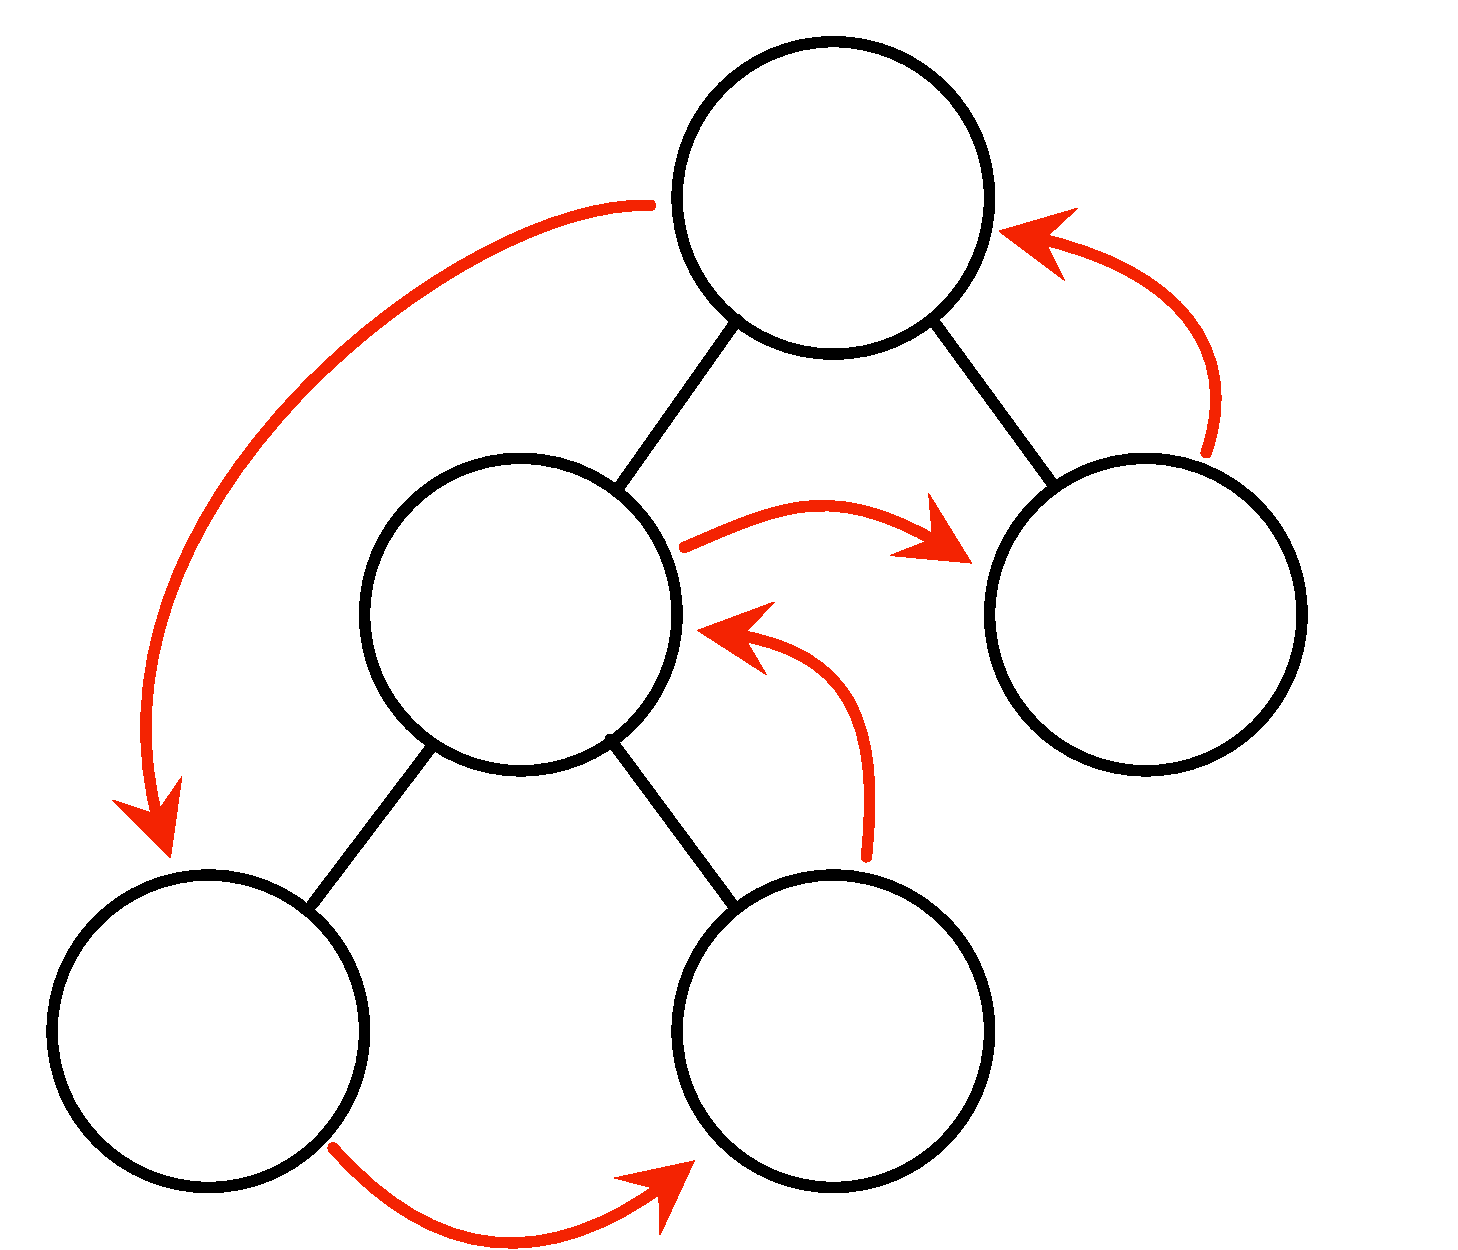
\includegraphics[width=.6\textwidth]{Images/TreeTraversal/Postorder.pdf}};
    \begin{scope}[x={(image.south east)},y={(image.north west)}]
    \begin{scope}[x={(image.south east)},y={(image.north west)}]
        \node at (0.57,0.83) {\large $1$};
        \node at (0.36,0.51) {\large $2$};
        \node at (0.78,0.51) {\large $3$};
        \node at (0.14,0.17) {\large $4$};
        \node at (0.57,0.17) {\large $5$};
    \end{scope}
    \end{scope}
\end{tikzpicture}}
         \caption{Diagram showing post-order tree traversal}
         \label{fig:Postorder}
     \end{subfigure}
          \hfill
     \begin{subfigure}[b]{0.45\textwidth}
         \centering
         \resizebox{\linewidth}{!}{\begin{tikzpicture}
    \node[anchor = south west,inner sep=0] (image) at (0,0) {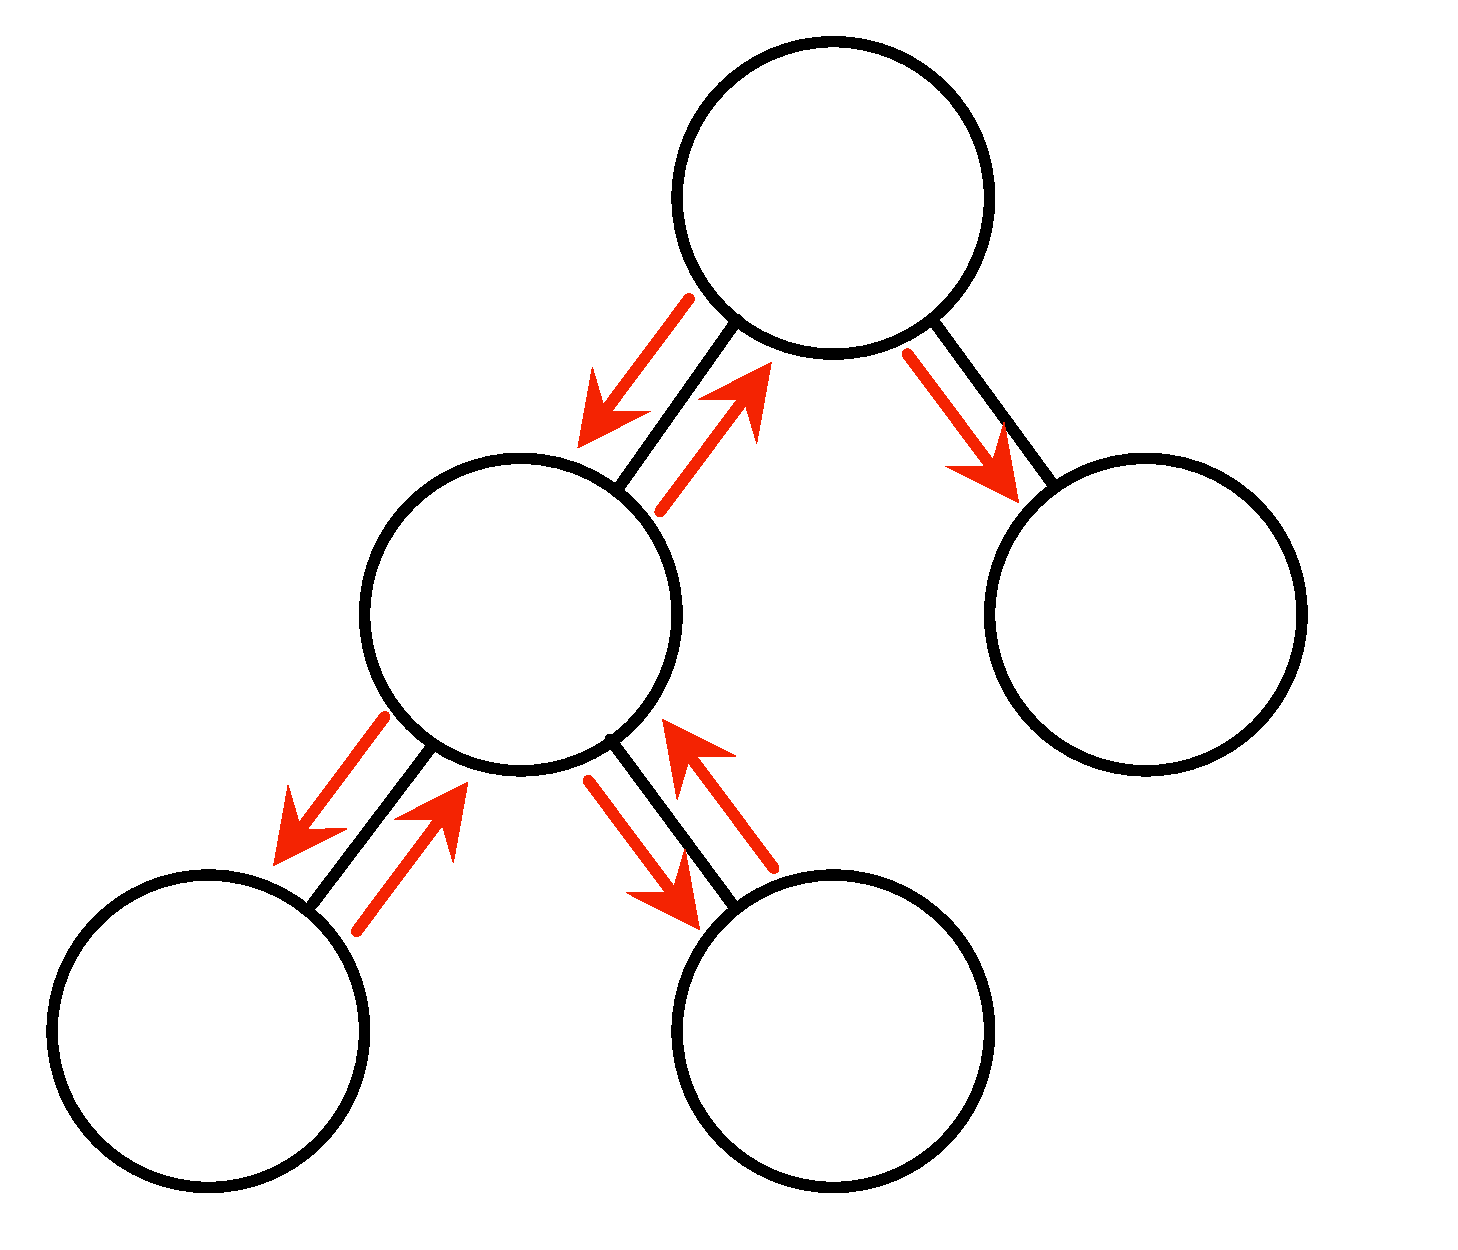
\includegraphics[width=.6\textwidth]{Images/TreeTraversal/Preorder.pdf}};
    \begin{scope}[x={(image.south east)},y={(image.north west)}]
    \begin{scope}[x={(image.south east)},y={(image.north west)}]
        \node at (0.57,0.83) {\large $1$};
        \node at (0.36,0.51) {\large $2$};
        \node at (0.78,0.51) {\large $3$};
        \node at (0.14,0.17) {\large $4$};
        \node at (0.57,0.17) {\large $5$};
    \end{scope}
    \end{scope}
\end{tikzpicture}}
         \caption{Diagram showing pre-order tree traversal}
         \label{fig:Preorder}
     \end{subfigure}
        \caption{Diagrams showing Pre and Post order traversal of the tree defined in \cref{fig:BlankTree}}
        \label{fig:TreeTraversal}
\end{figure}




\section{Condition number}\label{appendix:ConNum}


 \begin{figure}
     \centering
     Condition number of various matrices seen in the paper with $\epsilon=1e-1$
     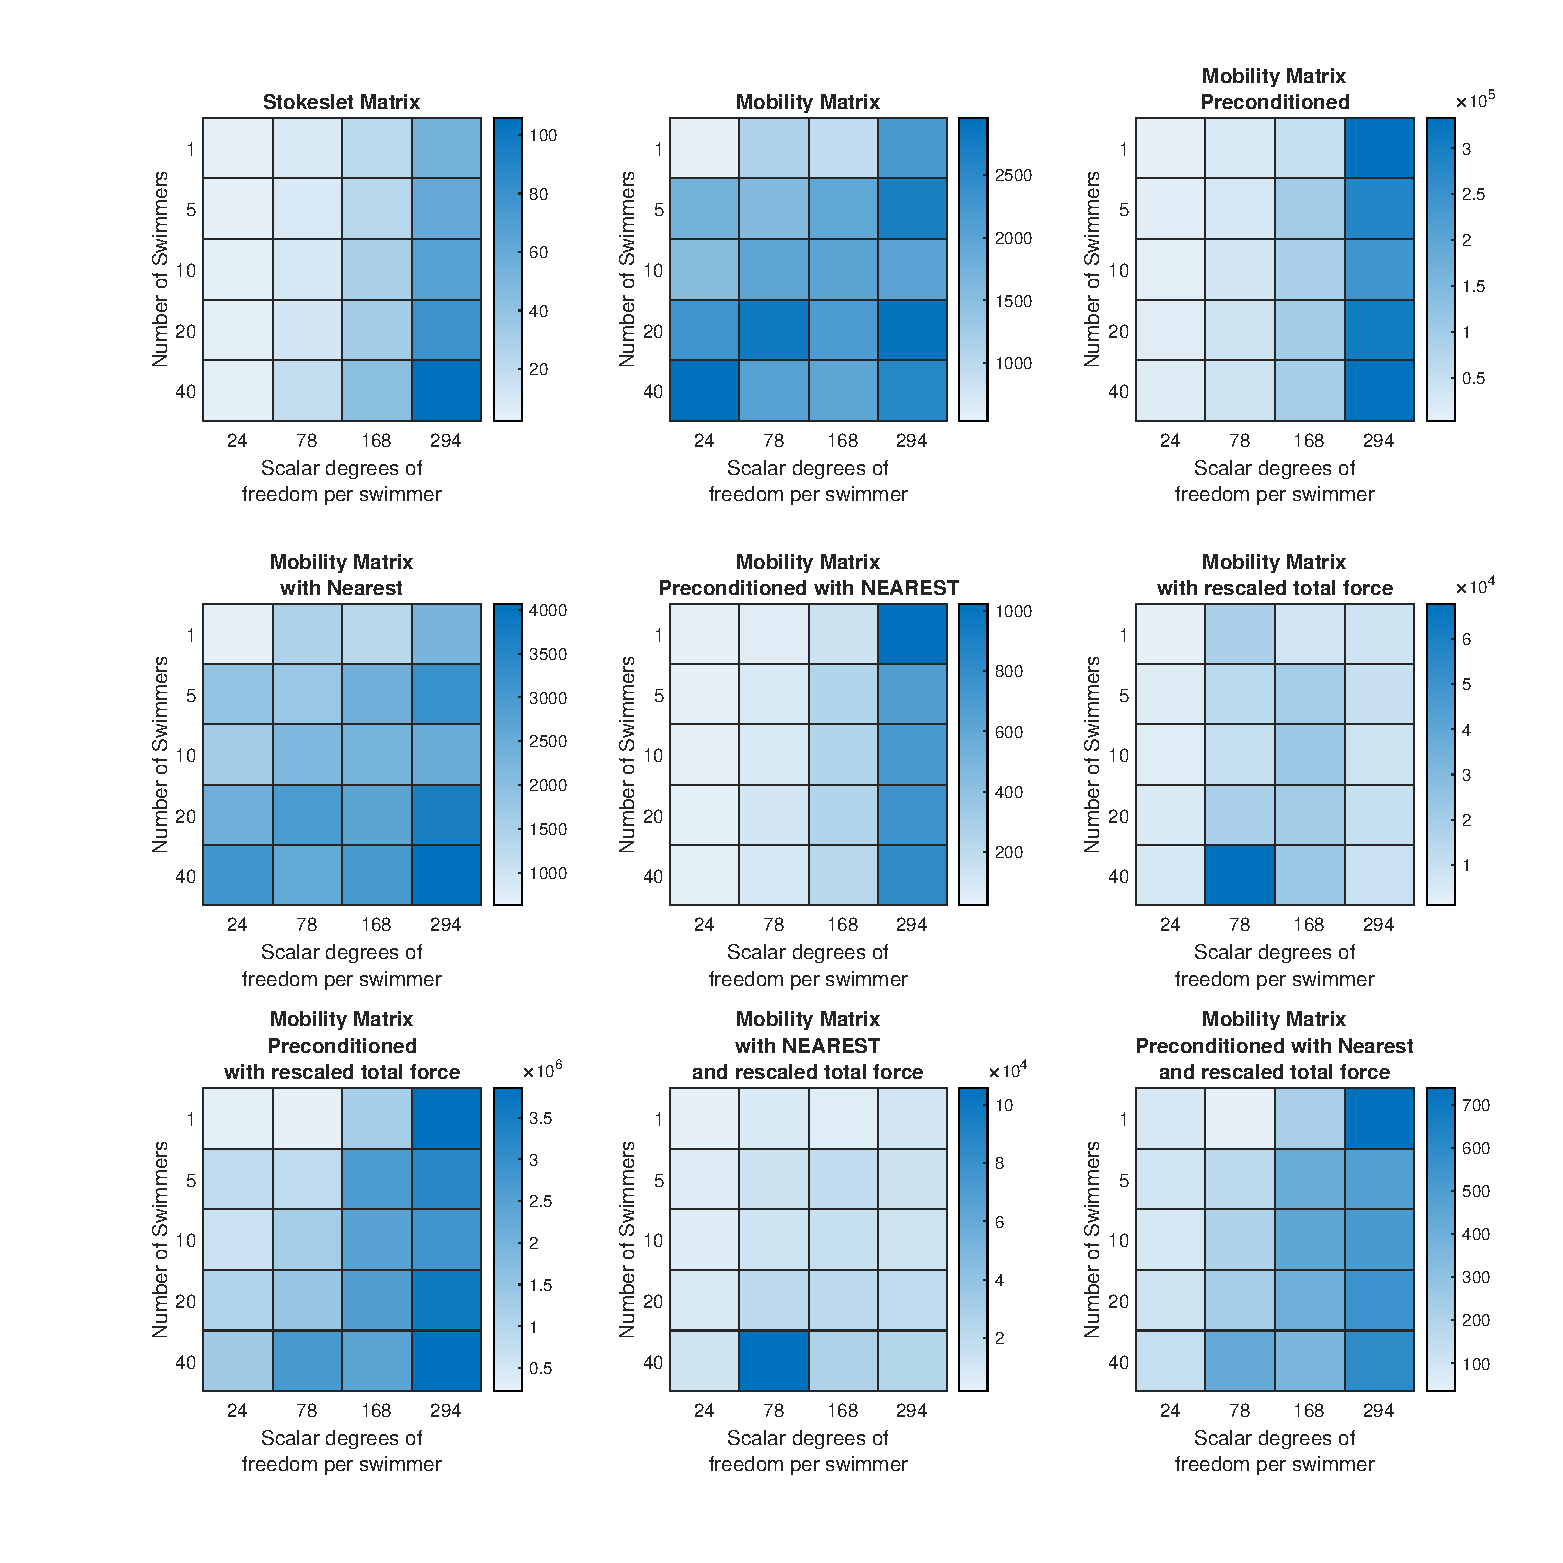
\includegraphics[width=0.6\textwidth]{Images/Condition/Condition-1.pdf}
     \caption{Caption}
     \label{fig:Condition1}
 \end{figure}
 \begin{figure}
 \ContinuedFloat
     \centering
     Condition number of various matrices seen in the paper with $\epsilon=1e-2$
     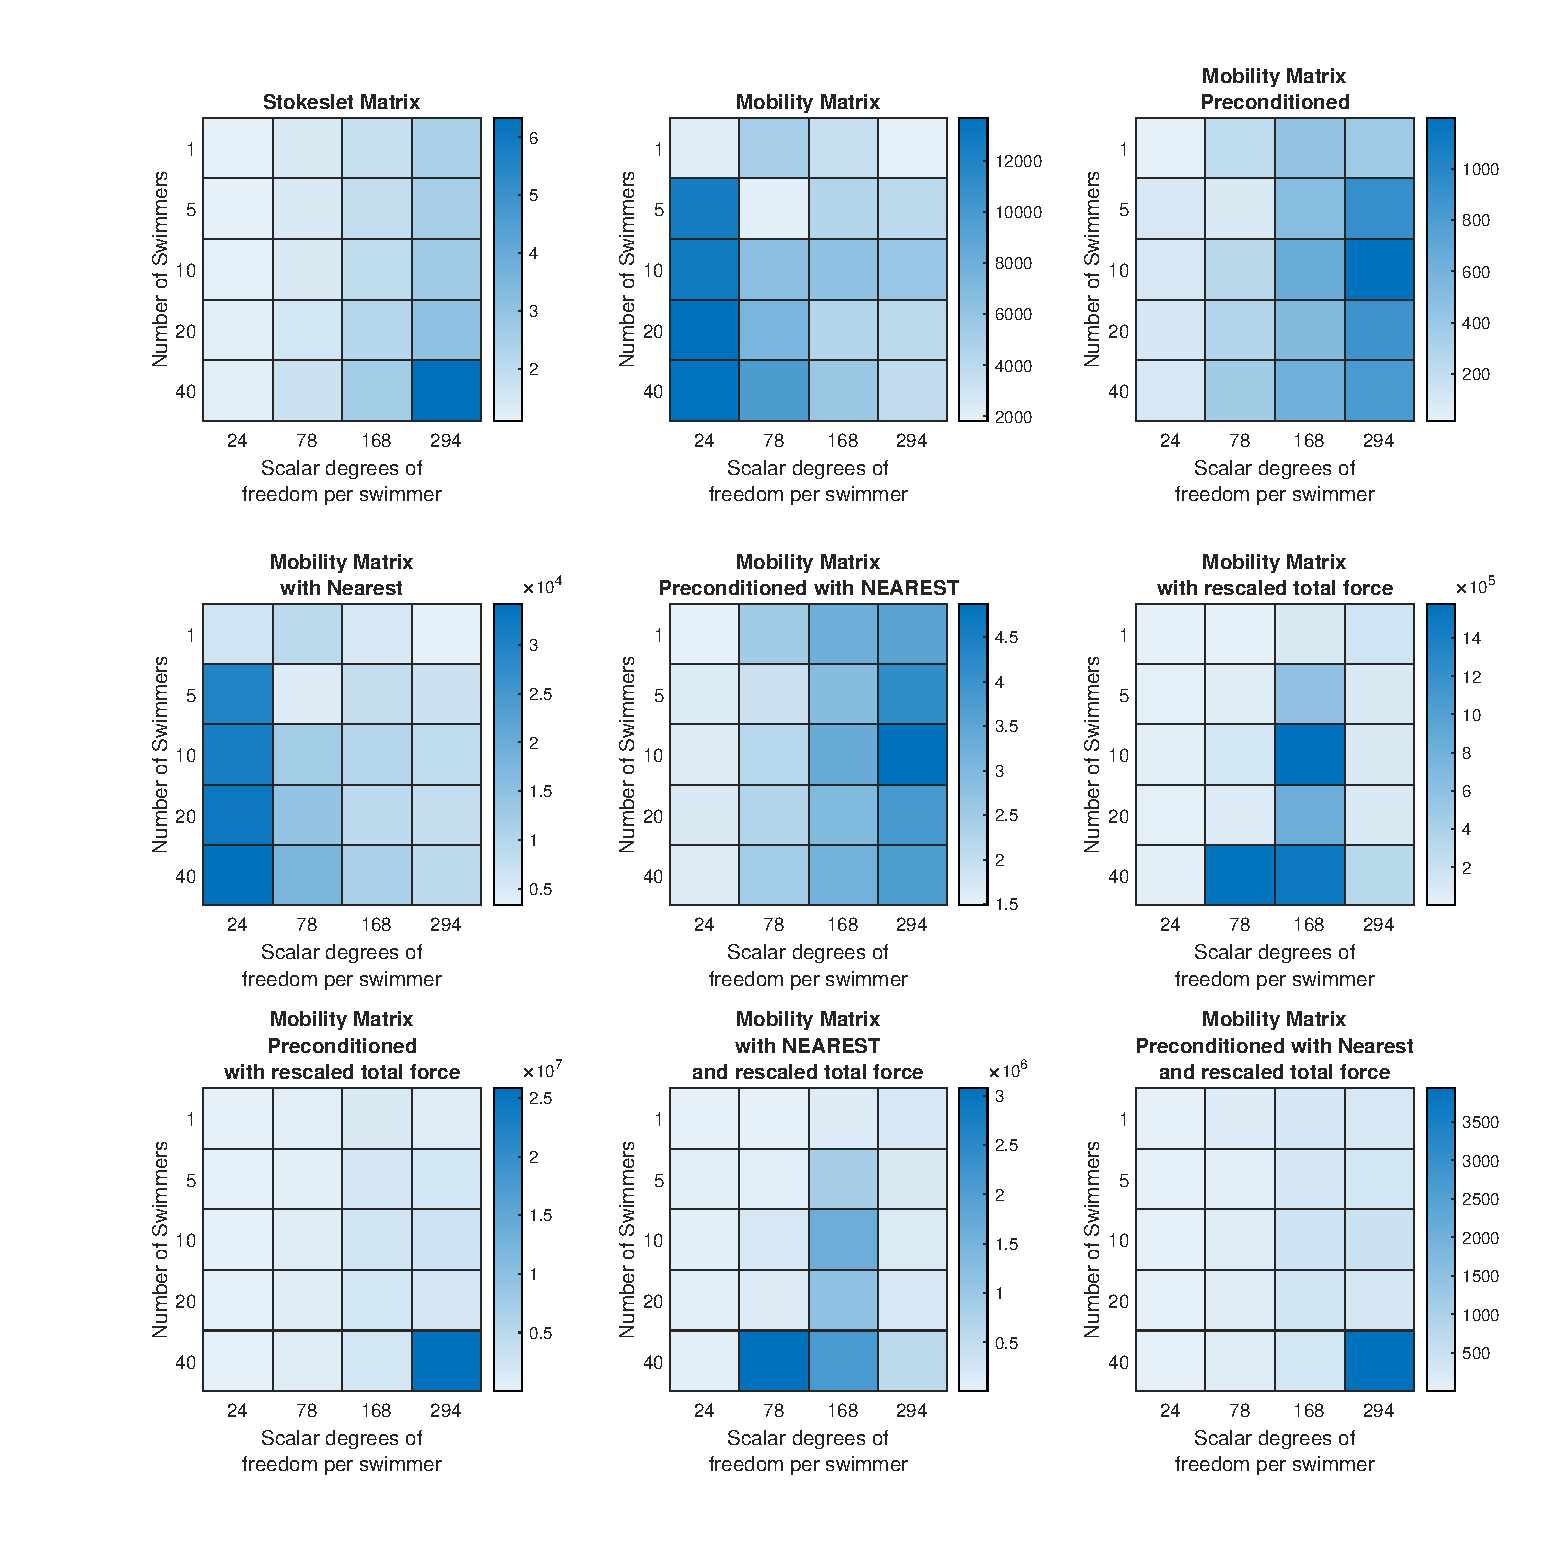
\includegraphics[width=0.6\textwidth]{Images/Condition/Condition-2.pdf}
     \caption{Caption}
     \label{fig:Condition2}
\end{figure}
\begin{figure}
\ContinuedFloat
     \centering
     Condition number of various matrices seen in the paper with $\epsilon=1e-5$
     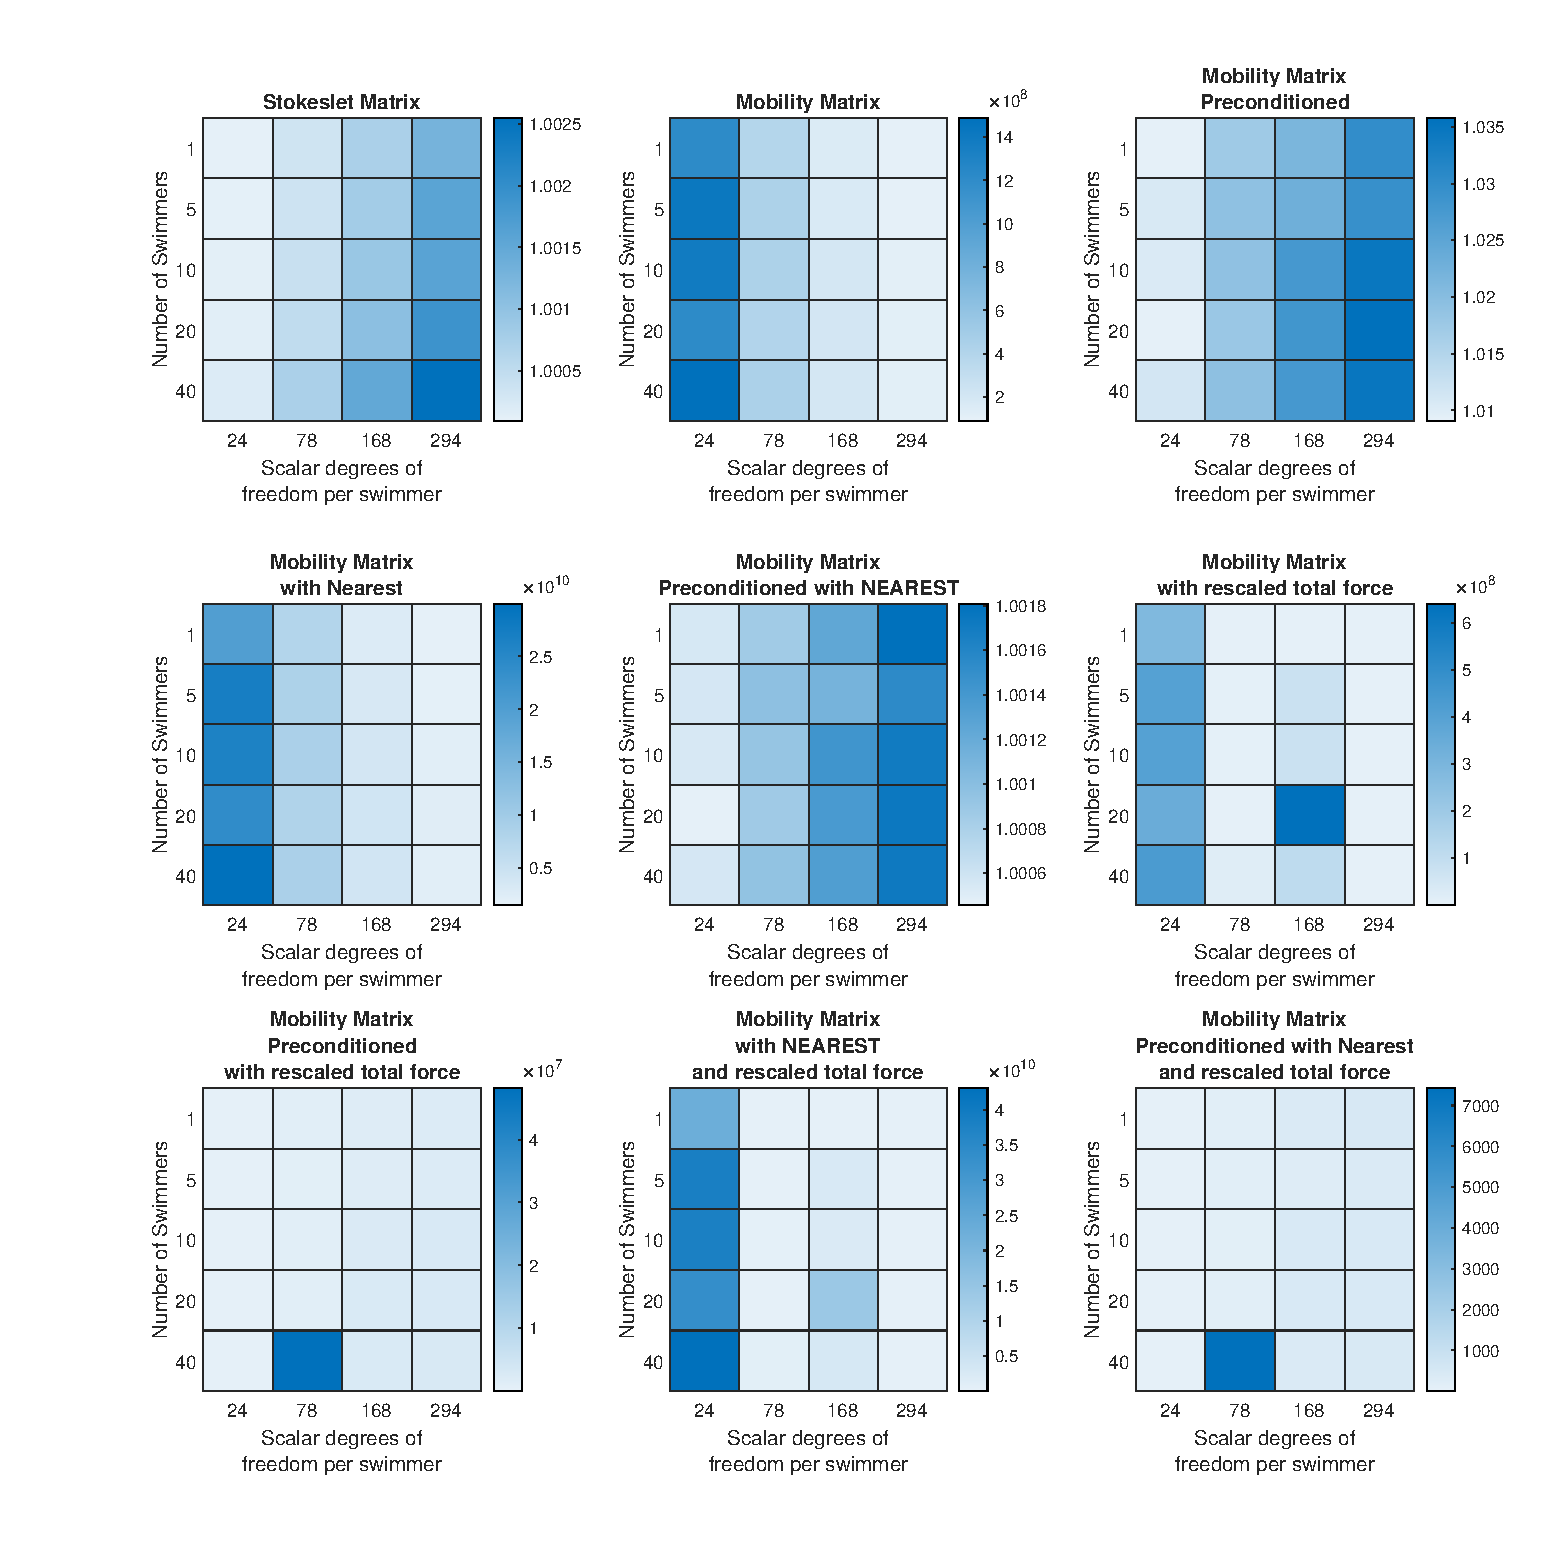
\includegraphics[width=0.6\textwidth]{Images/Condition/Condition-5.pdf}
     \caption{Caption}
     \label{fig:Condition5}
\end{figure}

 \begin{figure}
     \centering
     Eigenvalue plots of various matrices seen in the paper with $\epsilon=1e-1$
     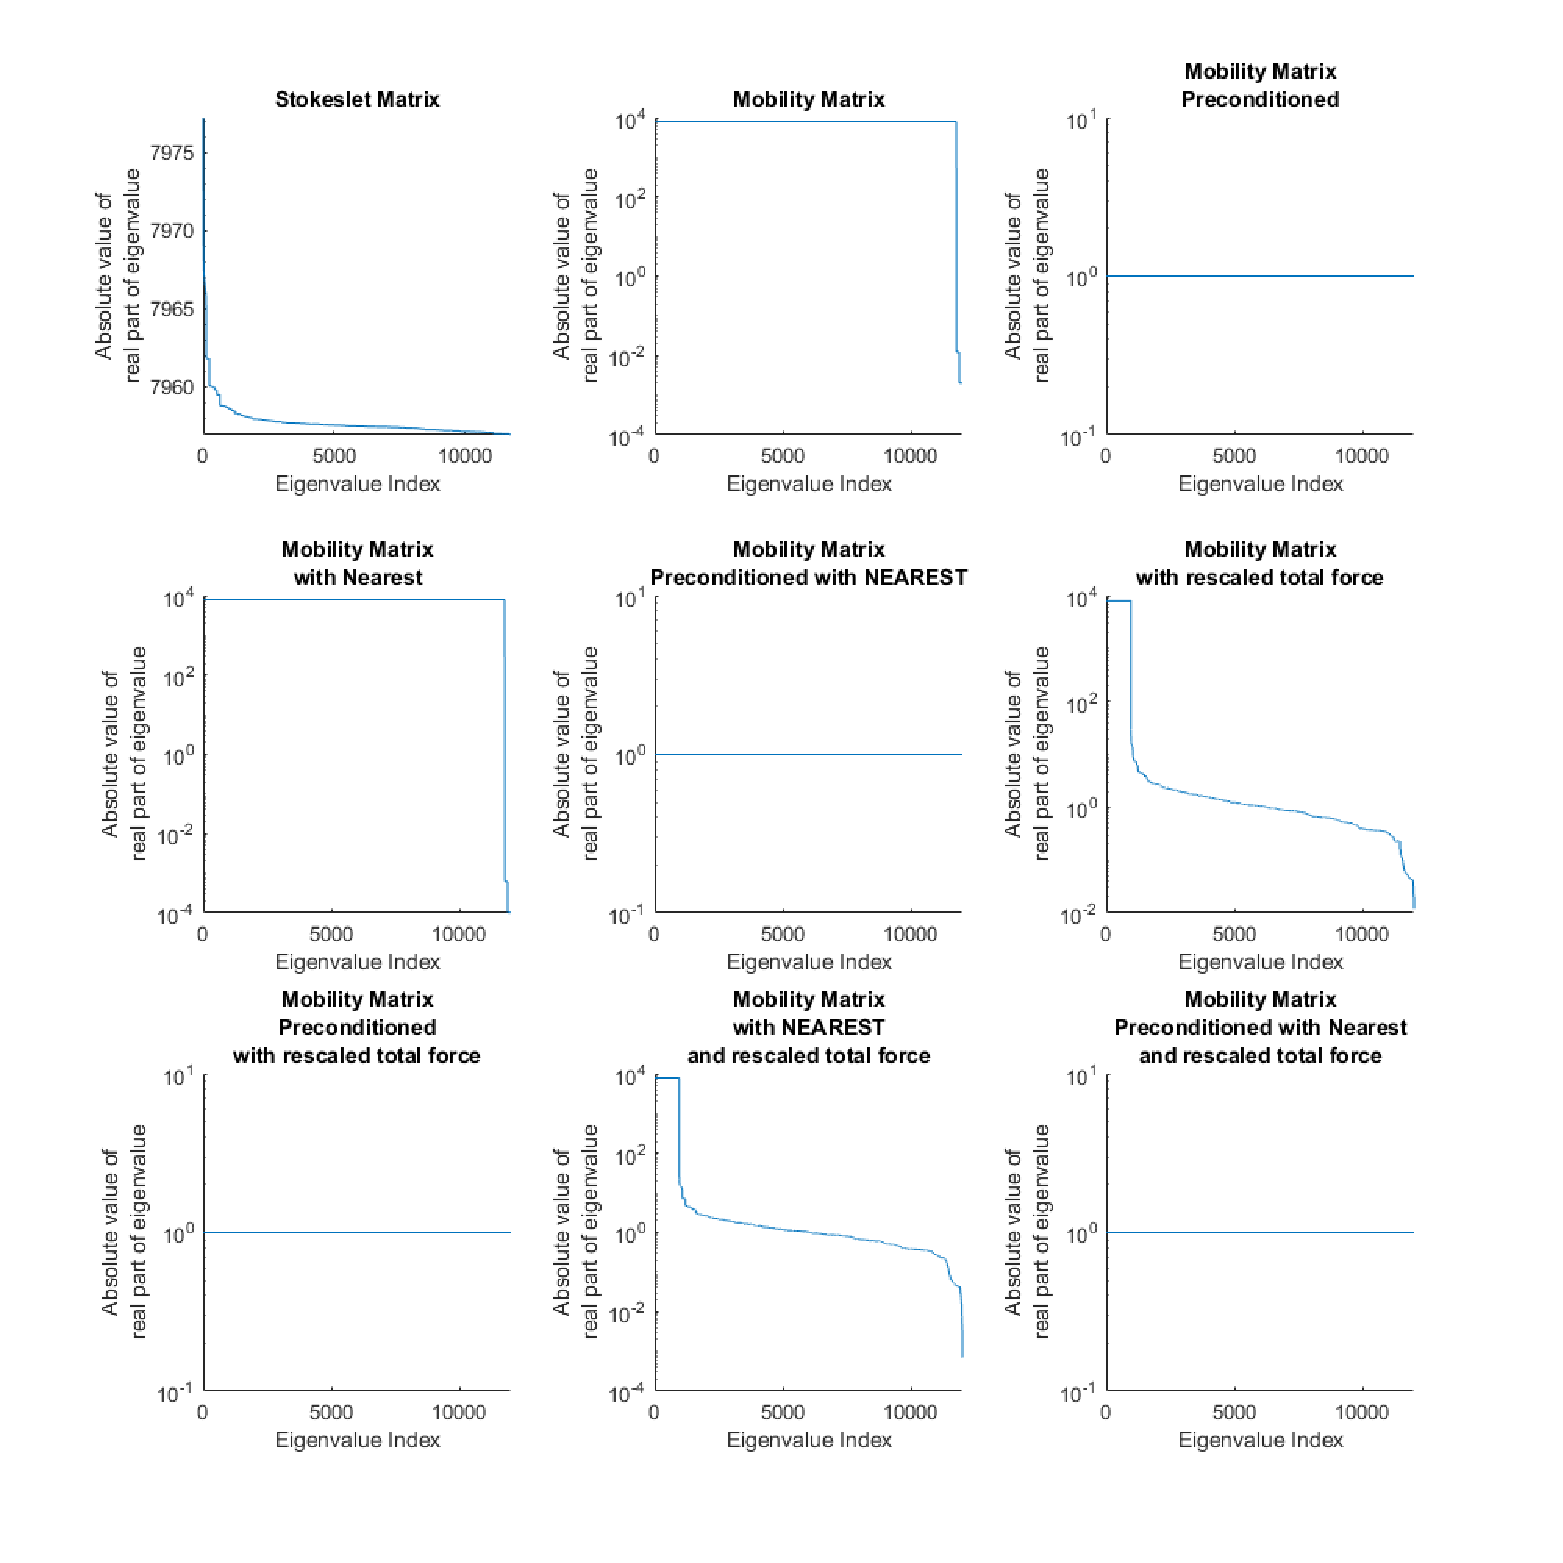
\includegraphics[width=0.6\textwidth]{Images/Eigenplots/EigenPlots-1.pdf}
     \caption{Caption}
     \label{fig:Eigen1}
 \end{figure}
 \begin{figure}
 \ContinuedFloat
     \centering
     Eigenvalue plots of various matrices seen in the paper with $\epsilon=1e-2$
     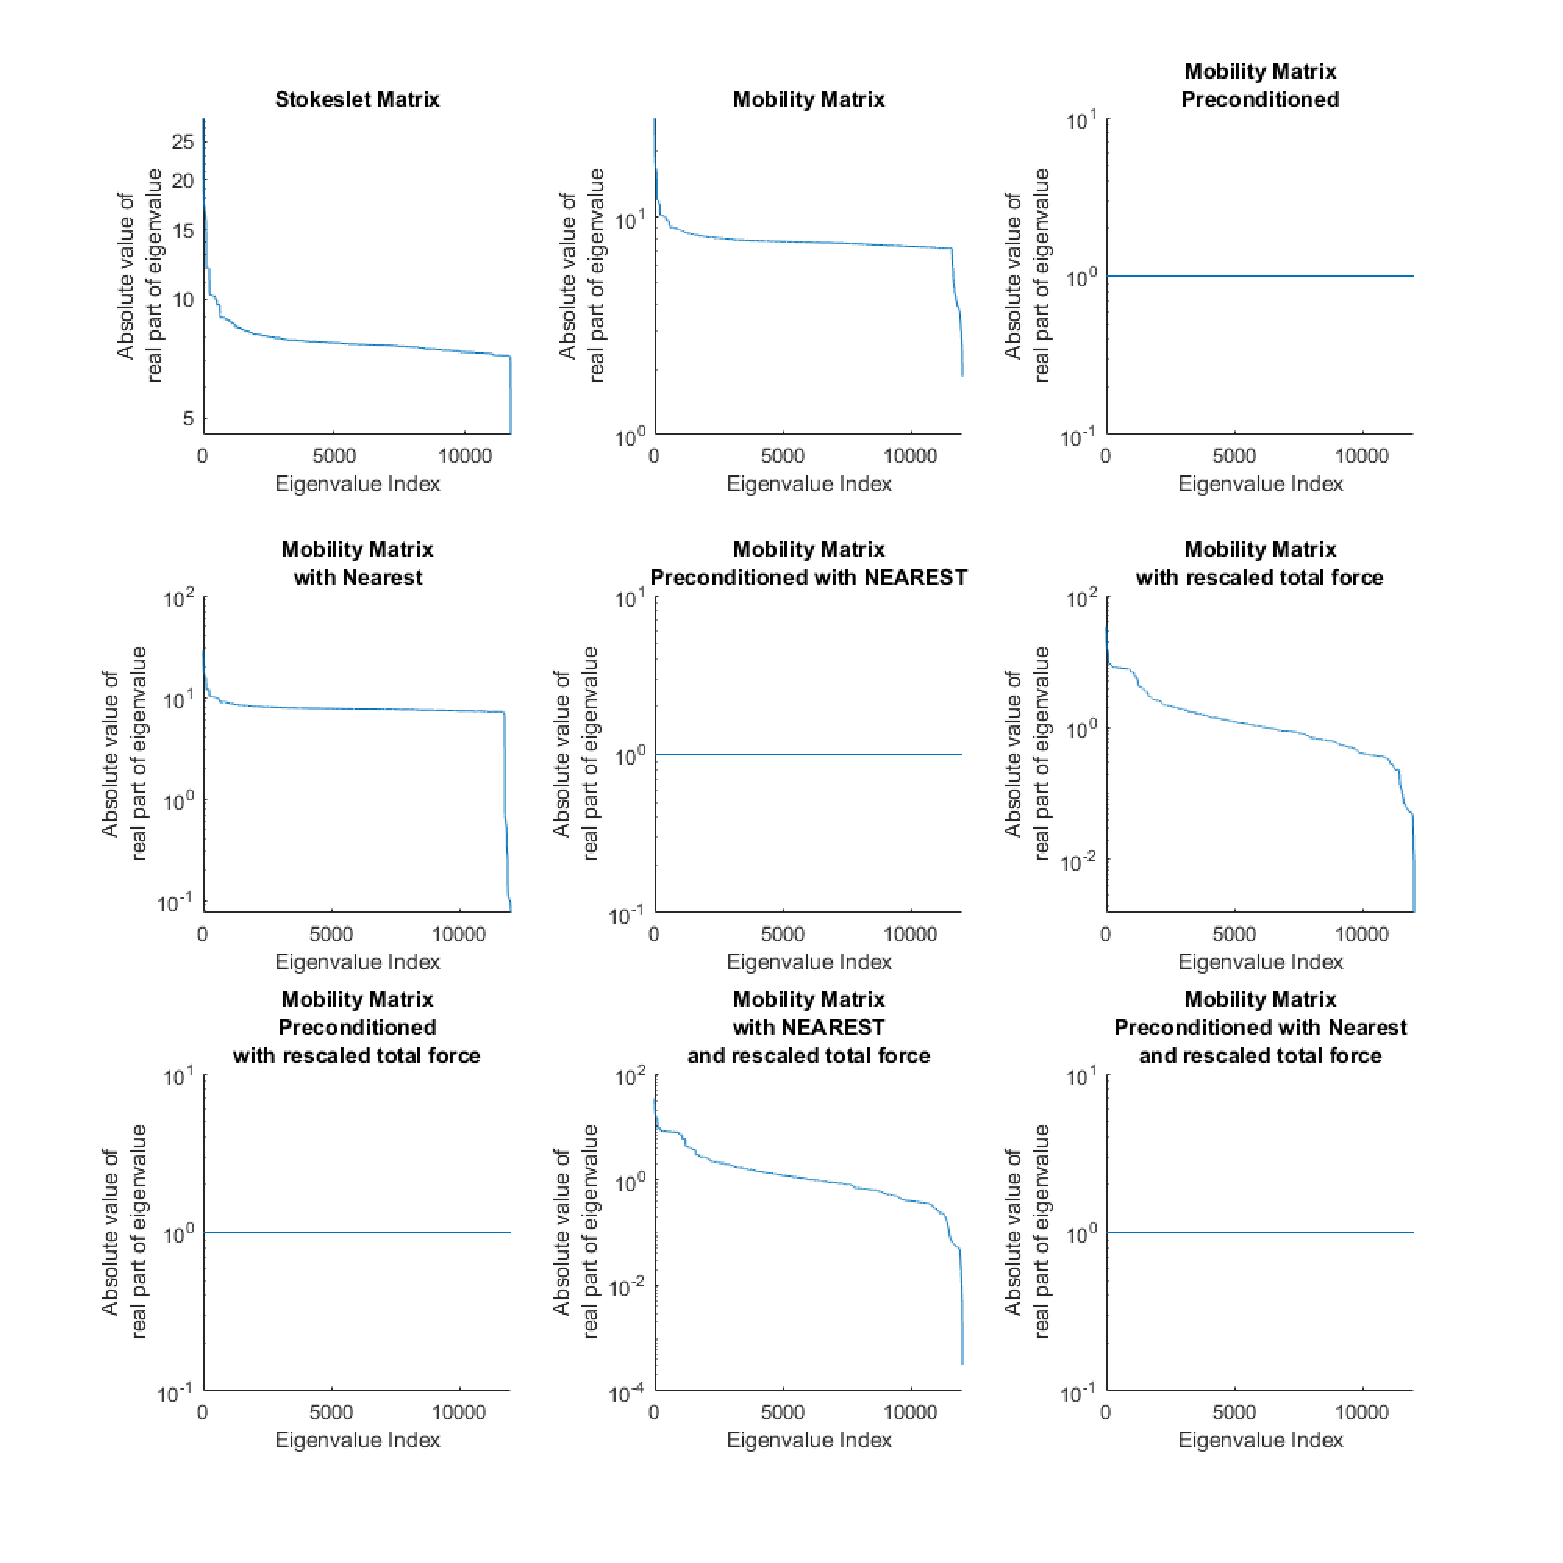
\includegraphics[width=0.6\textwidth]{Images/Eigenplots/EigenPlots-2.pdf}
     \caption{Caption}
     \label{fig:Eigen2}
\end{figure}
\begin{figure}
\ContinuedFloat
     \centering
     Eigenvalue plots of various matrices seen in the paper with $\epsilon=1e-5$
     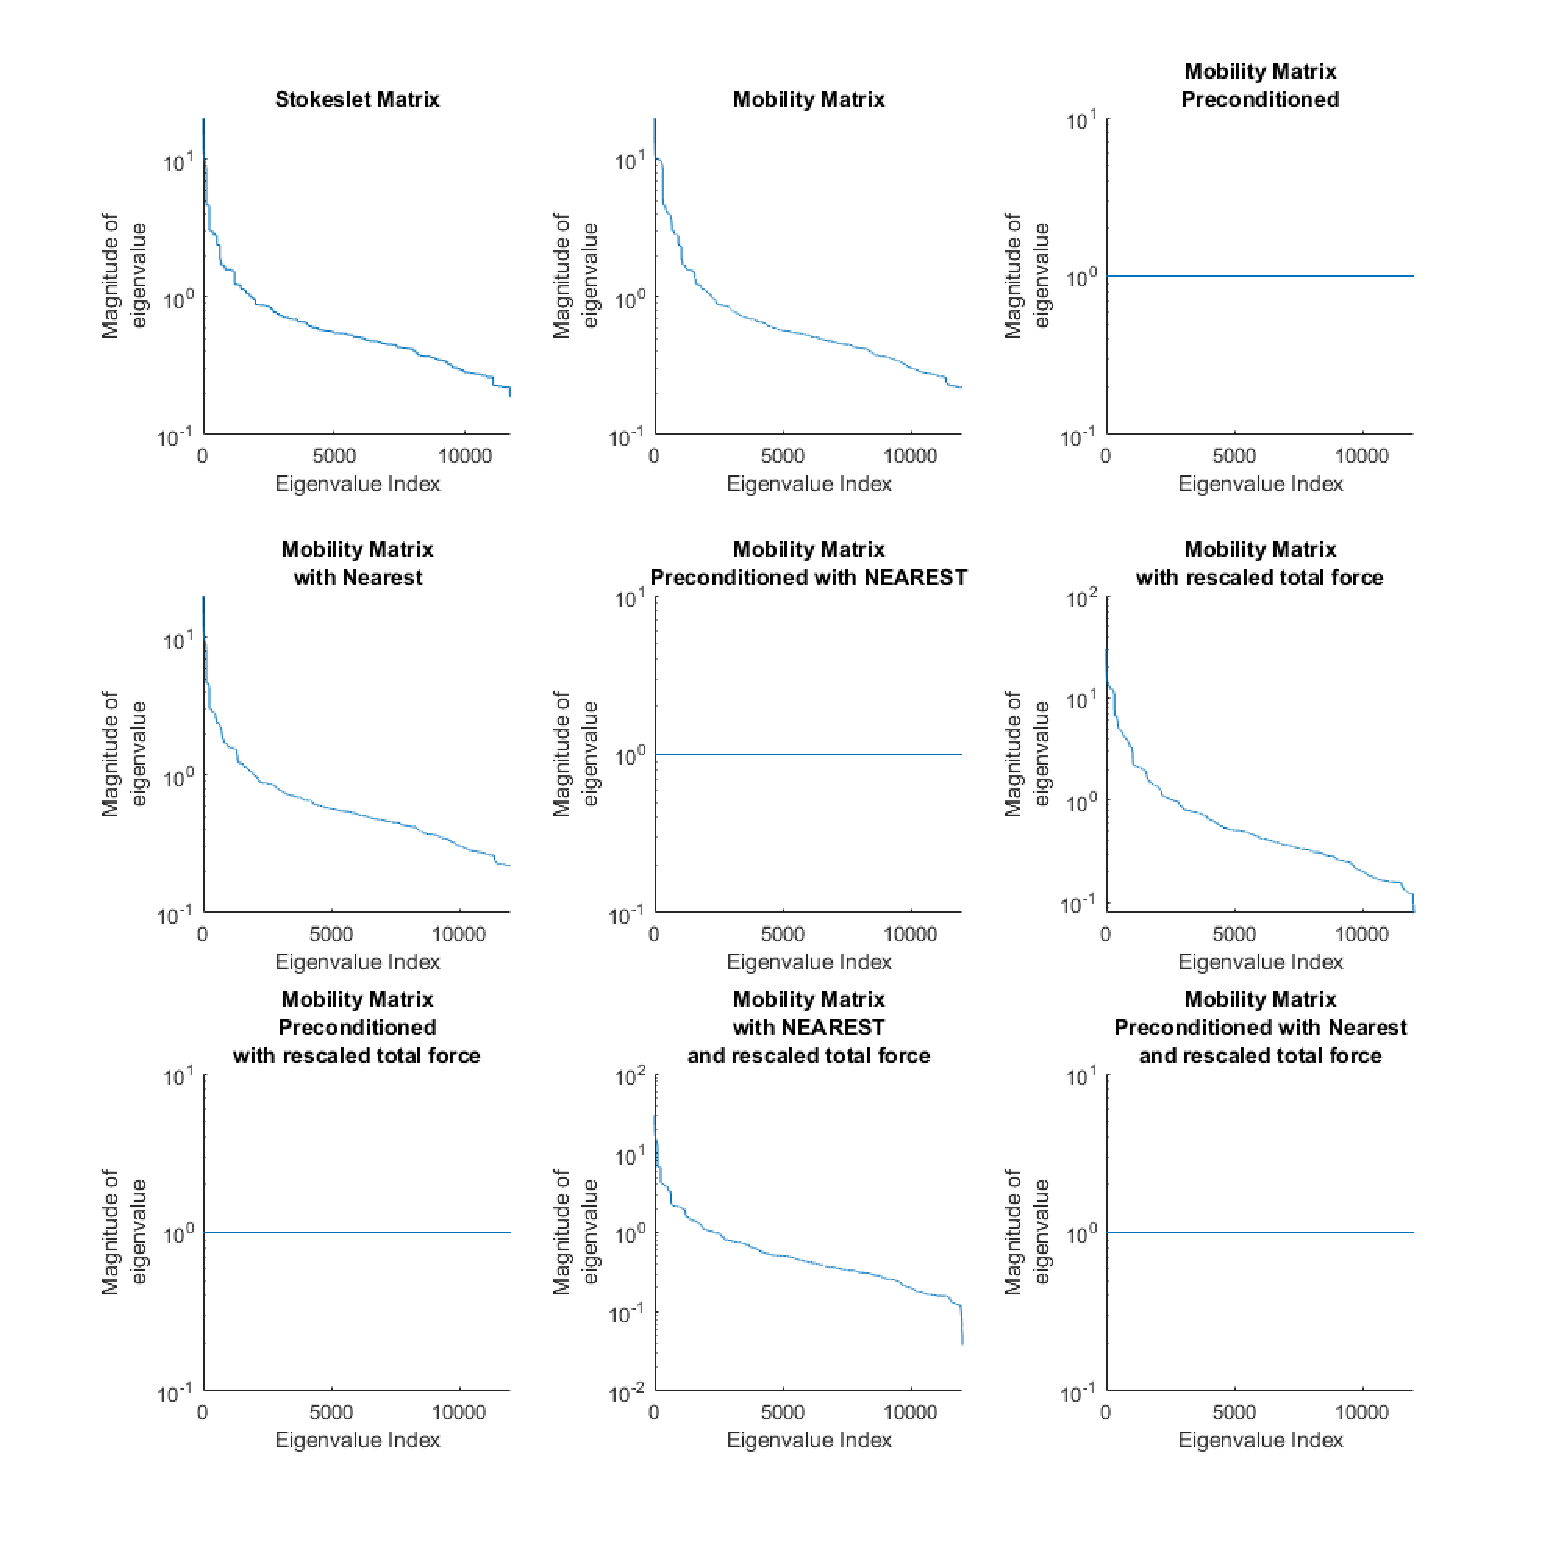
\includegraphics[width=0.6\textwidth]{Images/Eigenplots/EigenPlots-5.pdf}
     \caption{Caption}
     \label{fig:Eigen5}
\end{figure}

